%%%%%%%%%%%%%%%%%%%%%%%%%%%%%%%%%%%%%%%%%
% Class Notes Template
% LaTeX Template
% By: Ryan Grove
%%%%%%%%%%%%%%%%%%%%%%%%%%%%%%%%%%%%%%%%%

%----------------------------------------------------------------------------------------
%	PACKAGES AND OTHER DOCUMENT CONFIGURATIONS
%----------------------------------------------------------------------------------------

\documentclass[paper=a4, fontsize=11pt]{scrartcl} % A4 paper and 11pt font size

\usepackage[T1]{fontenc} % Use 8-bit encoding that has 256 glyphs
\usepackage{fourier} % Use the Adobe Utopia font for the document - comment this line to return to the LaTeX default
\usepackage[english]{babel} % English language/hyphenation
\usepackage{amsmath,amsfonts,amsthm} % Math packages

\usepackage{lipsum} % Used for inserting dummy 'Lorem ipsum' text into the template

\usepackage{sectsty} % Allows customizing section commands
\allsectionsfont{\centering \normalfont\scshape} % Make all sections centered, the default font and small caps

\usepackage{fancyhdr} % Custom headers and footers
\pagestyle{fancyplain} % Makes all pages in the document conform to the custom headers and footers
\fancyhead{} % No page header - if you want one, create it in the same way as the footers below
\fancyfoot[L]{} % Empty left footer
\fancyfoot[C]{} % Empty center footer
%\fancyfoot[R]{\thepage} % Page numbering for right footer
\renewcommand{\headrulewidth}{0pt} % Remove header underlines
\renewcommand{\footrulewidth}{0pt} % Remove footer underlines
\setlength{\headheight}{13.6pt} % Customize the height of the header

\numberwithin{equation}{section} % Number equations within sections (i.e. 1.1, 1.2, 2.1, 2.2 instead of 1, 2, 3, 4)
\numberwithin{figure}{section} % Number figures within sections (i.e. 1.1, 1.2, 2.1, 2.2 instead of 1, 2, 3, 4)
\numberwithin{table}{section} % Number tables within sections (i.e. 1.1, 1.2, 2.1, 2.2 instead of 1, 2, 3, 4)

\setlength\parindent{0pt} % Removes all indentation from paragraphs - comment this line for an assignment with lots of text

\usepackage{lastpage}
\usepackage{fancyhdr}
\cfoot{\thepage\ of \pageref{LastPage}}

\def\v{\hbox{$\mathbf v$}}
\def\w{\hbox{$\mathbf w$}}
\def\u{\hbox{$\mathbf u$}}
\def\x{\hbox{$\textbf{x}$}}
\def\z{\hbox{$\mathbf z$}}
\def\a{\hbox{$\mathbf a$}}
\def\b{\hbox{$\mathbf b$}}
\def\L{\hbox{$\mathcal L$}}
\def\C{\hbox{$\mathbb C$}}
\def\B{\hbox{$\mathcal B$}}
\def\R{\hbox{$\mathbb R$}}
\def\X{\hbox{$\underline X$}}
\def\Q{\hbox{$\mathbb Q$}}
\def\R{\hbox{$\mathbb R$}}
\def\N{\hbox{$\mathbb N$}}
\def\C{\hbox{$\mathbb C$}}
\def\0{\hbox{$\mathbf 0$}}
\def\Y{\hbox{$\underline Y$}}
\def\a{\hbox{$\mathbf a$}}
\def\u{\hbox{$\mathbf u$}}
\def\w{\hbox{$\mathbf w$}}
\def\y{\hbox{$\mathbf y$}}
\def\X{\hbox{$\underline X$}}
\def\dd{\hbox{$\partial $}}
\def\B{\hbox{$\mathcal B$}}
\def\F{\hbox{$\mathcal F$}}
\def\L{\hbox{$\mathcal L$}}
\def\M{\hbox{$\mathcal M$}}
\def\D{\hbox{$\mathscr {D}$}}
\def\RR{\hbox{$\mathscr{R}$}}
\def\I{\hbox{$\mathcal I$}}

\usepackage{amssymb}
%\theoremstyle{plain}
\usepackage[margin = .75in]{geometry}
\newtheorem{claim}{Claim}
\newtheorem{theorem}{Theorem}[section]
\newtheorem{lemma}[theorem]{Lemma}
\newtheorem{proposition}[theorem]{Proposition}
\newtheorem{corollary}[theorem]{Corollary}
\newtheorem{problem}[theorem]{Problem}
%\theoremstyle{definition}
\newtheorem{definition}[theorem]{Definition}
%\theoremstyle{remark}
\newtheorem{remark}[theorem]{Remark}
\newtheorem{remarks}[theorem]{Remarks}
\newtheorem{example}[theorem]{Example}
\newcommand{\ds}{\displaystyle}
\newcommand{\ZZ}{\mathbb{Z}}
\newcommand{\QQ}{\mathbb{Q}}
\newcommand{\e}{\varepsilon}
\newcommand{\bbf}{\textbf}
\newcommand{\p}{\parallel}
\usepackage{color}
\newcommand{\field}[1]{\mathbb{#1}}
\usepackage{amsmath}
\usepackage{amsthm}
\usepackage{amssymb}
\usepackage{mathrsfs}
\usepackage{cancel}
\usepackage{upgreek}
\usepackage{graphicx}
\usepackage{multirow}
\usepackage{setspace}
\usepackage{url}
\usepackage{subfigure}
\usepackage{enumerate}
\usepackage{cases}
\usepackage{mathrsfs}
\usepackage{rotating}

%----------------------------------------------------------------------------------------
%	TITLE SECTION
%----------------------------------------------------------------------------------------

\newcommand{\horrule}[1]{\rule{\linewidth}{#1}} % Create horizontal rule command with 1 argument of height

\title{	
\normalfont \normalsize 
\textsc{Ryan Grove, Clemson University, MATH1080 - 9} \\ [25pt] % Your name, university, class
\horrule{0.5pt} \\[0.4cm] % Thin top horizontal rule
\huge Section 7.7: Approximate Integration \\ % The assignment title
\horrule{2pt} \\[0.5cm] % Thick bottom horizontal rule
}

\author{Date:} % The due date

\date{\normalsize February 9, 2016} % A custom date

\begin{document}

\maketitle % Print the title

\begin{flushleft}
\begin{tabular}{l l}
Name: \rule{3.2in}{.01cm}  & {}%Table number: \rule{1in}{.01cm}\\
\end{tabular}
\end{flushleft}

%----------------------------------------------------------------------------------------
%	Lecture
%----------------------------------------------------------------------------------------

\section*{\textbf{Lecture:}}

It is impossible to find the exact value of a definite integral, $\ds\int_a^b f(x) dx$, in two situations.\\
\indent

\textbf{Situation 1}: It is difficult, or even impossible, to find an antiderivative of $f$.
\begin{quote}
\flushleft
\hspace{0.53in} Examples: \quad \quad \quad $\ds\int_0^1 e^{x^2}dx \quad \hspace{0.25in} \text{ or } \hspace{0.25in} \quad \ds\int_{-1}^1 \ds\sqrt{1+x^3}dx$
\end{quote}
\indent

\textbf{Situation 2}: The function $f$ is determined from a scientific experience through instrument readings or collected data and there is no formula for the function.\\
\indent

\indent\\

In both cases we need to find \underline{\hspace{1.25in}} values of definite integrals. We already know one such method. Recall that the definite integral is defined as a \underline{\hspace{1in}} of \underline{\hspace{1.25in}} sums, so any Riemann sum could be used as an approximation to the integral:\\
\indent

\begin{quote}
\flushleft If we divide $[a,b]$ into $n$ subintervals of equal length $\Delta x = \underline{\hspace{.75in}}$, then we have

\[\ds\int_a^b f(x) dx \approx \ds\sum_{i=1}^n f(x_i^*) \Delta x\]

where $x_i^*$ is any point in the $i^{\text{th}}$ subinterval $[x_{i-1},x_i]$.\\
\end{quote}
\indent
\newpage
\textbf{\underline{Left Endpoint Approximation}}:\\
\indent

\[\ds\int_a^b f(x) dx \approx L_n = \ds\sum_{i=1}^n f(x_{i-1})\Delta x \hspace{3in}\]
\vspace{-75pt} \[\hspace{3in} 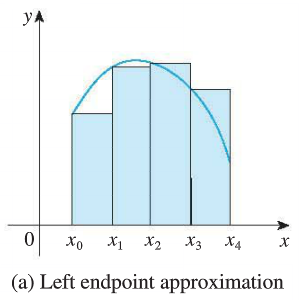
\includegraphics[scale=0.45]{7-7pic1.png}\]
\indent

\textbf{\underline{Right Endpoint Approximation}}:\\
\indent

\[\ds\int_a^b f(x) dx \approx R_n = \ds\sum_{i=1}^n f(x_i)\Delta x \hspace{3in}\] \vspace{-75pt}
\[\hspace{3in} 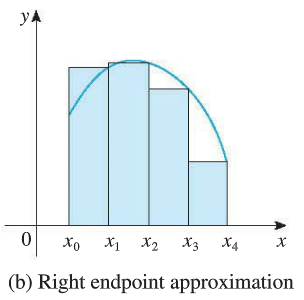
\includegraphics[scale=0.45]{7-7pic2.png}\]
\indent

\fbox{
  \parbox{\textwidth}{
  \vspace{5pt} \textbf{\underline{Midpoint Rule}}:
  
  \[\ds\int_a^b f(x) dx \approx M_n = \ds\sum_{i=1}^n f(\bar{x}_i)\Delta x \hspace{3in}\]
  
  \hspace{0.25in} where $\bar{x}_i = \ds\frac{x_{i-1}+x_i}{2} = \text{ midpoint of } [x_{i-1},x_i]$\\
  
  \hspace{0.25in} and $\Delta x = \ds\frac{b-a}{n}$.\\
  
  \vspace{-150pt}
  \[\hspace{3in} 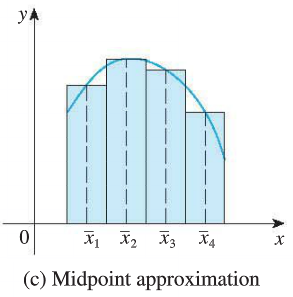
\includegraphics[scale=0.45]{7-7pic3.png}\]
  
  }}
  \indent\\
  \indent
  
  Another approximation, called the \textbf{Trapezoidal Rule}, results from averaging the Left and Right Endpoint approximations:
  \begin{align*}
  \ds\int_a^b f(x) dx &\approx \ds\frac{1}{2}\bigg[ \ds\sum_{i=1}^n f(x_{i-1})\Delta x + \ds\sum_{i=1}^n f(x_i)\Delta x\bigg] = \ds\frac{\Delta x}{2} \bigg[\ds\sum_{i=1}^n \left(f(x_{i-1}) + f(x_i)\right)\bigg]\\
  &= \ds\frac{\Delta x}{2}\bigg[\left(f(x_0) + f(x_1)\right) + \left(f(x_1) + f(x_2)\right) + \cdots + \left(f({x_n-1}) + f(x_n)\right)\bigg]\\
  &= \ds\frac{\Delta x}{2}\bigg[f(x_0) + 2f(x_1) + 2f(x_2) + \cdots + 2f(x_{n-1}) + f(x_n)\bigg]
  \end{align*}
  \indent
  \newpage
  \fbox{
  \parbox{\textwidth}{
  \vspace{5pt} \textbf{\underline{Trapezoid Rule}}:
  
  \[\ds\int_a^b f(x) dx \approx T_n = \ds\frac{\Delta x}{2} \bigg[f(x_0) + 2f(x_1) + 2f(x_2) + \cdots + 2f(x_{n-1}) + f(x_n)\bigg]\]
  
  \hspace{0.25in} where $\Delta x = \ds\frac{b-a}{n}$ and $x_i=a+i\Delta x$.\\
  
  }}
  \indent\\
  \indent
  
  
 The reason for the name Trapezoidal Rule can be seen from Figure 2, which illustrates the case with $f(x)\geq 0$ and $n=4$. \\
 \indent\\
 \indent
 
  The area of the trapezoid that lies above the $iˆ{\text{th}}$ subinterval is
 
 \[\Delta x \left(\ds\frac{f(x_{i-1} + f(x_i)}{2}\right) = \ds\frac{\Delta x}{2}[f(x_{i-1}) + f(x_i)]\hspace{3in}\]
 
 and if we add the areas of all these trapezoids,\\
 we get the Trapezoidal Rule approximation.\\

 
 \vspace{-145pt}  
 \[\hspace{4.25in} 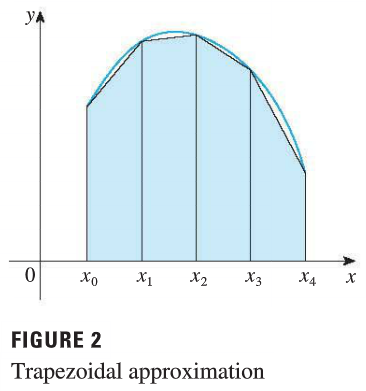
\includegraphics[scale=0.45]{7-7pic4.png}\]
 \indent
 
 The following table shows the results of various appproximations for $\ds\int_1^2 \ds\frac{1}{x}dx$.\\
 
 \[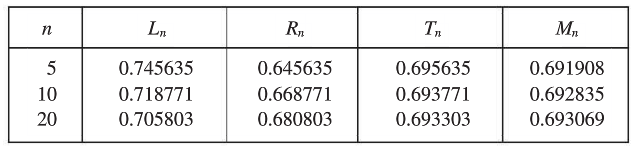
\includegraphics[scale=0.49]{7-7table1.png}\]

 
 \underline{Example 1}: Use $(a)$ the Trapezoidal Rule and $(b)$ the Midpoint Rule with $n=5$ to approximate the integral $\ds\int_1^2 \ds\frac{1}{x} dx$.\\
 \indent

\vspace{4.5in}

\[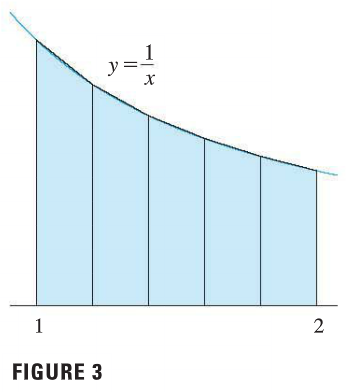
\includegraphics[scale=0.45]{7-7pic5.png} \hspace{1in} 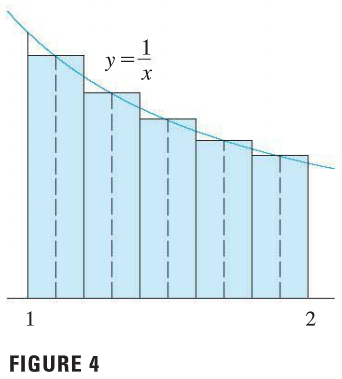
\includegraphics[scale=0.45]{7-7pic6.png}\]



In Example 1, we deliberately chose an integral whose value can be computed explicitly so that we can see how accurate the Trapezoidal and Midpoint Rules are. We have,\\

\[\ds\int_1^2 \ds\frac{1}{x}\text{ } dx = \hspace{3.5in}\]
\indent

The \underline{\hspace{1in}} in using an approximation is defined to be the amount that needs to be added to the approximation to make it exact (i.e. \textbf{error} $=$ \textbf{exact} $-$ \textbf{approximation}). From the values in Example 1 we see that the errors in the Trapezoidal and Midpoint Rule approximations for $n=5$ are
\[E_T\approx -0.003488 \quad \text{ and } \quad E_M \approx 0.001239\]


In general, we have

\[E_T = \ds\int_a^b f(x) dx - T_n \quad \text{ and } \quad E_M = \ds\int_a^b f(x) dx - M_n\]

The following tables show the results of calculations similar to those in Example 1, but for $n=5, 10, \text{ and } 20$ and for the left and right endpoint approximations as well as the Trapezoidal and Midpoint Rules.\\
\indent

\underline{Observations}:

\begin{enumerate}
\item In all of the methods we get more accurate approximations when we increase the value of $n$.
\item The errors in the left and right endpoint approximations are opposite in sign and appear to decrease by a factor of about 2 when we double the value of $n$
\item The Trapezoidal and Midpoint Rules are much more accurate than the endpoint approximations.
\item The errors in the Trapezoidal and Midpoint Rules are opposite in sign and appear to decrease by a factor of about 4 when we double the value of $n$.
\item The size of the error in the Midpoint Rule is about half the size of the error in the Trapezoidal Rule.\\
\end{enumerate}

\[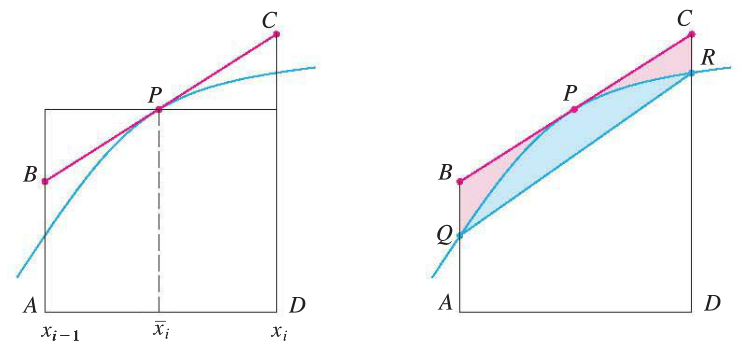
\includegraphics[scale=0.45]{7-7pic7.png}\]
\indent

These observations are corroborated in the following error estimates, which are proved in books on numerical analysis. \\
\indent

\fbox{
  \parbox{\textwidth}{
  \vspace{5pt} \textbf{\underline{Error Bounds}}: Suppose $|f''(x)|\leq K$ for $a\leq x \leq b$. If $E_T$ and $E_M$ are the errors in the Trapezoidal and Midpoint Rules, then
  \[|E_T| \leq \ds\frac{K(b-a)^3}{12n^2} \quad \text{ and } \quad |E_M| \leq \ds\frac{K(b-a)^3}{24n^2}\]
  
  }}
  \indent\\
  \indent
  
  \underline{Example 1 revisited...}:\\
 \indent
  
  Let's apply this error estimate to the Trapezoidal Rule approximation in Example 1 where $f(x) = \ds\frac{1}{x}$.\\
  \indent
  
  \vspace{4in}
  
  Comparing this error estimate of 0.006667 with the actual error of about 0.002488, we see that it can happen that the actual error is substantially less than the upper bound for the error given by the above formula.\\
  \indent
  
  \newpage
  \underline{Example 2}: How large should we take $n$ in order to guarantee that the Trapezoidal and Midpoint Rule approximations for $\ds\int_1^2 \ds\frac{1}{x} dx$ are accurate to within 0.0001?\\
  \indent
  
  \vspace{3.5in}
  
  
  \section*{Simpson's Rule}
  Another rule for approximate integration results from using \underline{\hspace{1.25in}} instead of straight line segments to approximate a curve. \\
  \indent
  
  As before, we divide $[a,b]$ into $n$ subintervals of equal length $h=\Delta x = \ds\frac{b-a}{n}$, but this time we assume that $n$ is an \textit{even} number. Then on each consecutive pair of intervals we approximate the curve $y=f(x)\geq 0$ by a parabola as shown in Figure 7. If $y_i=f(x_i)$, then $P_i(x_i,y_i)$ is the point on the curve lying above $x_i$. A typical parabola passes through three consecutive points $P_i, P_{i+1}, P_{i+2}$.\\
  \indent
  
  \[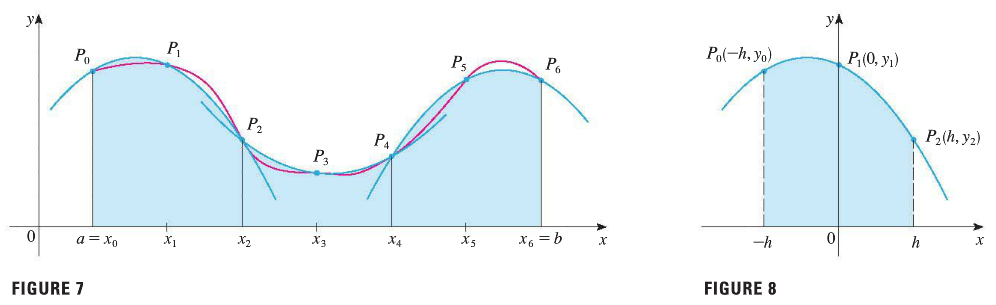
\includegraphics[scale=0.45]{7-7pic8.png}\]
  \indent
  
\fbox{
  \parbox{\textwidth}{
  \vspace{5pt}  \textbf{\underline{Simpson's Rule}}:
  \[\ds\int_a^b f(x) dx \approx S_n = \ds\frac{\Delta x }{3}\bigg[f(x_0) + 4f(x_1) + 2 f(x_2) + 4f(x_3) + \cdots + 2f(x_{n-2}) + 4 f(x_{n-1}) + f(x_n)\bigg]\]
  
  
  \hspace{0.25in} where $n$ is even and $\Delta x = \ds\frac{b-a}{n}$.\\
  
  }}
  \indent\\
  \indent
  
  
  
  \underline{Example 3}: Use Simpson's Rule with $n=10$ to approximate $\ds\int_1^2\ds\frac{1}{x} dx$.\\
  \indent
  
  \textbf{SOLUTION}: Putting $f(x)=\ds\frac{1}{x}, n=10$, and $\Delta x = 0.1$ in Simpson's Rule, we obtain
  
 \begin{align*}
 \ds\int_1^2\ds\frac{1}{x}dx &\approx S_{10}\\
 &= \ds\frac{\Delta x}{3}\bigg[f(1) + 4f(1.1) + 2f(1.2) + 4f(1.3) + \cdots + 2f(1.8) + 4f(1.9) + f(2)\bigg]\\
 \text{ }\\
 &= \hspace{3in}
 \text{ }\\
 \text{ }\\
 &\approx 0.6931250.\\
 \end{align*}
 
% The following table shows how Simpson's Rule compares with the Trapezoidal Rule and Midpoint Rule for the integral $\ds\int_1^2 \ds\frac{1}{x}dx = \ln 2\approx 0.693147\ldots$.\\
% 
% \[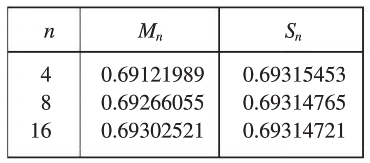
\includegraphics[scale=0.5]{7-7pic11.png}\]
  
  Notice that Simpson's Rule gives us a \textit{much better} approximation to the true value of the integral $(\ln 2\approx 0.693147\ldots)$ than does the Trapezoidal Rule ($T_{10} \approx 0.693771$) or the Midpoint Rule ($M_{10}\approx 0.692835$). It turns out that the approximations in Simpson's Rule are weighted averages of those in The Trapezoidal and Midpoint Rules, i.e.:
  
  \[S_{2n} = \frac{1}{3}T_n + \frac{2}{3}M_n\]
  
%  We can also observe how error, $E_S$, in Simpson's Rule decreases by a factor of about 16 when $n$ is doubled. That is consistent with the appearance of $n^4$ in the denominator of the following error estimate for Simpson's Rule, which is similar to the estimates given for the Trapezoidal and Midpoint Rules, but uses the fourth derivative of $f$.\\
%  \indent
%  
%\fbox{
%  \parbox{\textwidth}{
%  \vspace{5pt} \textbf{\underline{Error Bound for Simpson's Rule}}: Suppose that $|f^{(4)}(x)| \leq K$ for $a\leq x \leq b$. If $E_S$ is the error involved in using Simpson's Rule, then
%  \[|E_S|\leq \ds\frac{K(b-a)^5}{180n^4}\]
%  
%  }}
%  \indent\\
%  \indent
  
  
%  \underline{Example 5}: Figure 9 shows data traffic on the link from the United States to SWITCH, the Swiss academic and research network, on February 10, 1998. $D(t)$ is the data throughput, measured in megabits per second (Mb/s). Use Simpson's Rule to estimate the total amount of data transmitted on the link from midnight to noon on that day.\\
%  
%  \[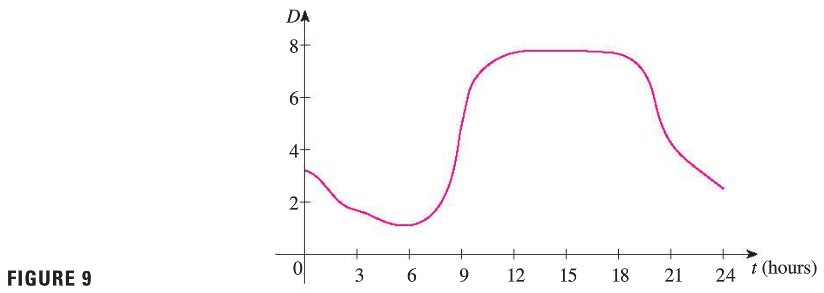
\includegraphics[scale=0.5]{7-7pic9.png}\]
%  \indent
  
  
%  \underline{Example 6}: How large should we take $n$ in order to guarantee that the Simpson's Rule approximation for $\ds\int_1^2\ds\frac{1}{x}dx$ is accurate to within 0.0001?\\
%  \indent
%  
%  
%  \vspace{3.5in}
%  
%  (Compare this with Example 2, where we obtained $n=41$ for the Trapezoidal Rule and $n=29$ for the Midpoint Rule.)\\
%  
\indent\\
 
  \underline{Example 4}: Use the listed rule with $n=10$ to approximate the integral $\ds\int_0^1 e^{x^2}dx$.
  \begin{enumerate}
  \item[(a)] Trapezoidal Rule
  
  \newpage
  
  \item[(b)] Midpoint Rule
  
  \vspace{4.5in}
  \item[(c)] Simpson's Rule
  \end{enumerate}
%  \item[(b)] Estimate the error involved in this approximation.\\
%  \end{enumerate}
  \indent
  
  
  

%\fbox{
%  \parbox{\textwidth}{
%  \vspace{5pt}


















%----------------------------------------------------------------------------------------

\end{document}